\chapter{x86 Explained}
\label{chapter:usecase}

\thomasrk[inline]{Mieux faire sentir que x86 est un exemple parmi tant d'autres,
  mais qu'il est très représentatif des difficultés que l'on peut rencontrer
  avec les HSE.}

At the time of writing this thesis\,\footnote{Spring 2018.}, the \emph{Intel 64
  and IA-32 Architectures Software Developer’s Manual} is 4842 pages long.
%
The output of \texttt{lshw -short} on one regular computer lists about 30
hardware components in addition to the main CPU.
%
Each of them come with its own documentations, often in the form of large
datasheets.
%
This means the information about how the computing platform works are scattered
throughout many sources.
%
This situation inevitably complicates the work of low-level software developers.
%
From a security perspective, they need to have a comprehensive view of how the
computing platform works as a whole.
%
This problematic also exists for hardware designers.
%
When they want to add a new feature, or a new component, they have to be certain
they will not break existing properties of the architecture by doing so.

This Chapter intends to give the readers a general overview of the x86
architecture, so that they can understand the challenge related to
hardware-based security enforcement with the x86 hardware architecture.
%
It proceeds as follows:
%
we describe in more detail how a typical x86 computer works, which kind of
hardware components are involved and how they interact with each others
(Section\,\ref{sec:usecase:architecture});
%
we focus on the key role played by the firmware in the platform functioning and
security (Section\,\ref{sec:usecase:firmware});
%
we detail several HSE mechanisms implemented by the firmware, including how they
have been compromised (Section\,\ref{sec:usecase:hse}).

\section{x86 Architecture Explained}
\label{sec:usecase:architecture}

\begin{figure}
  \centering
  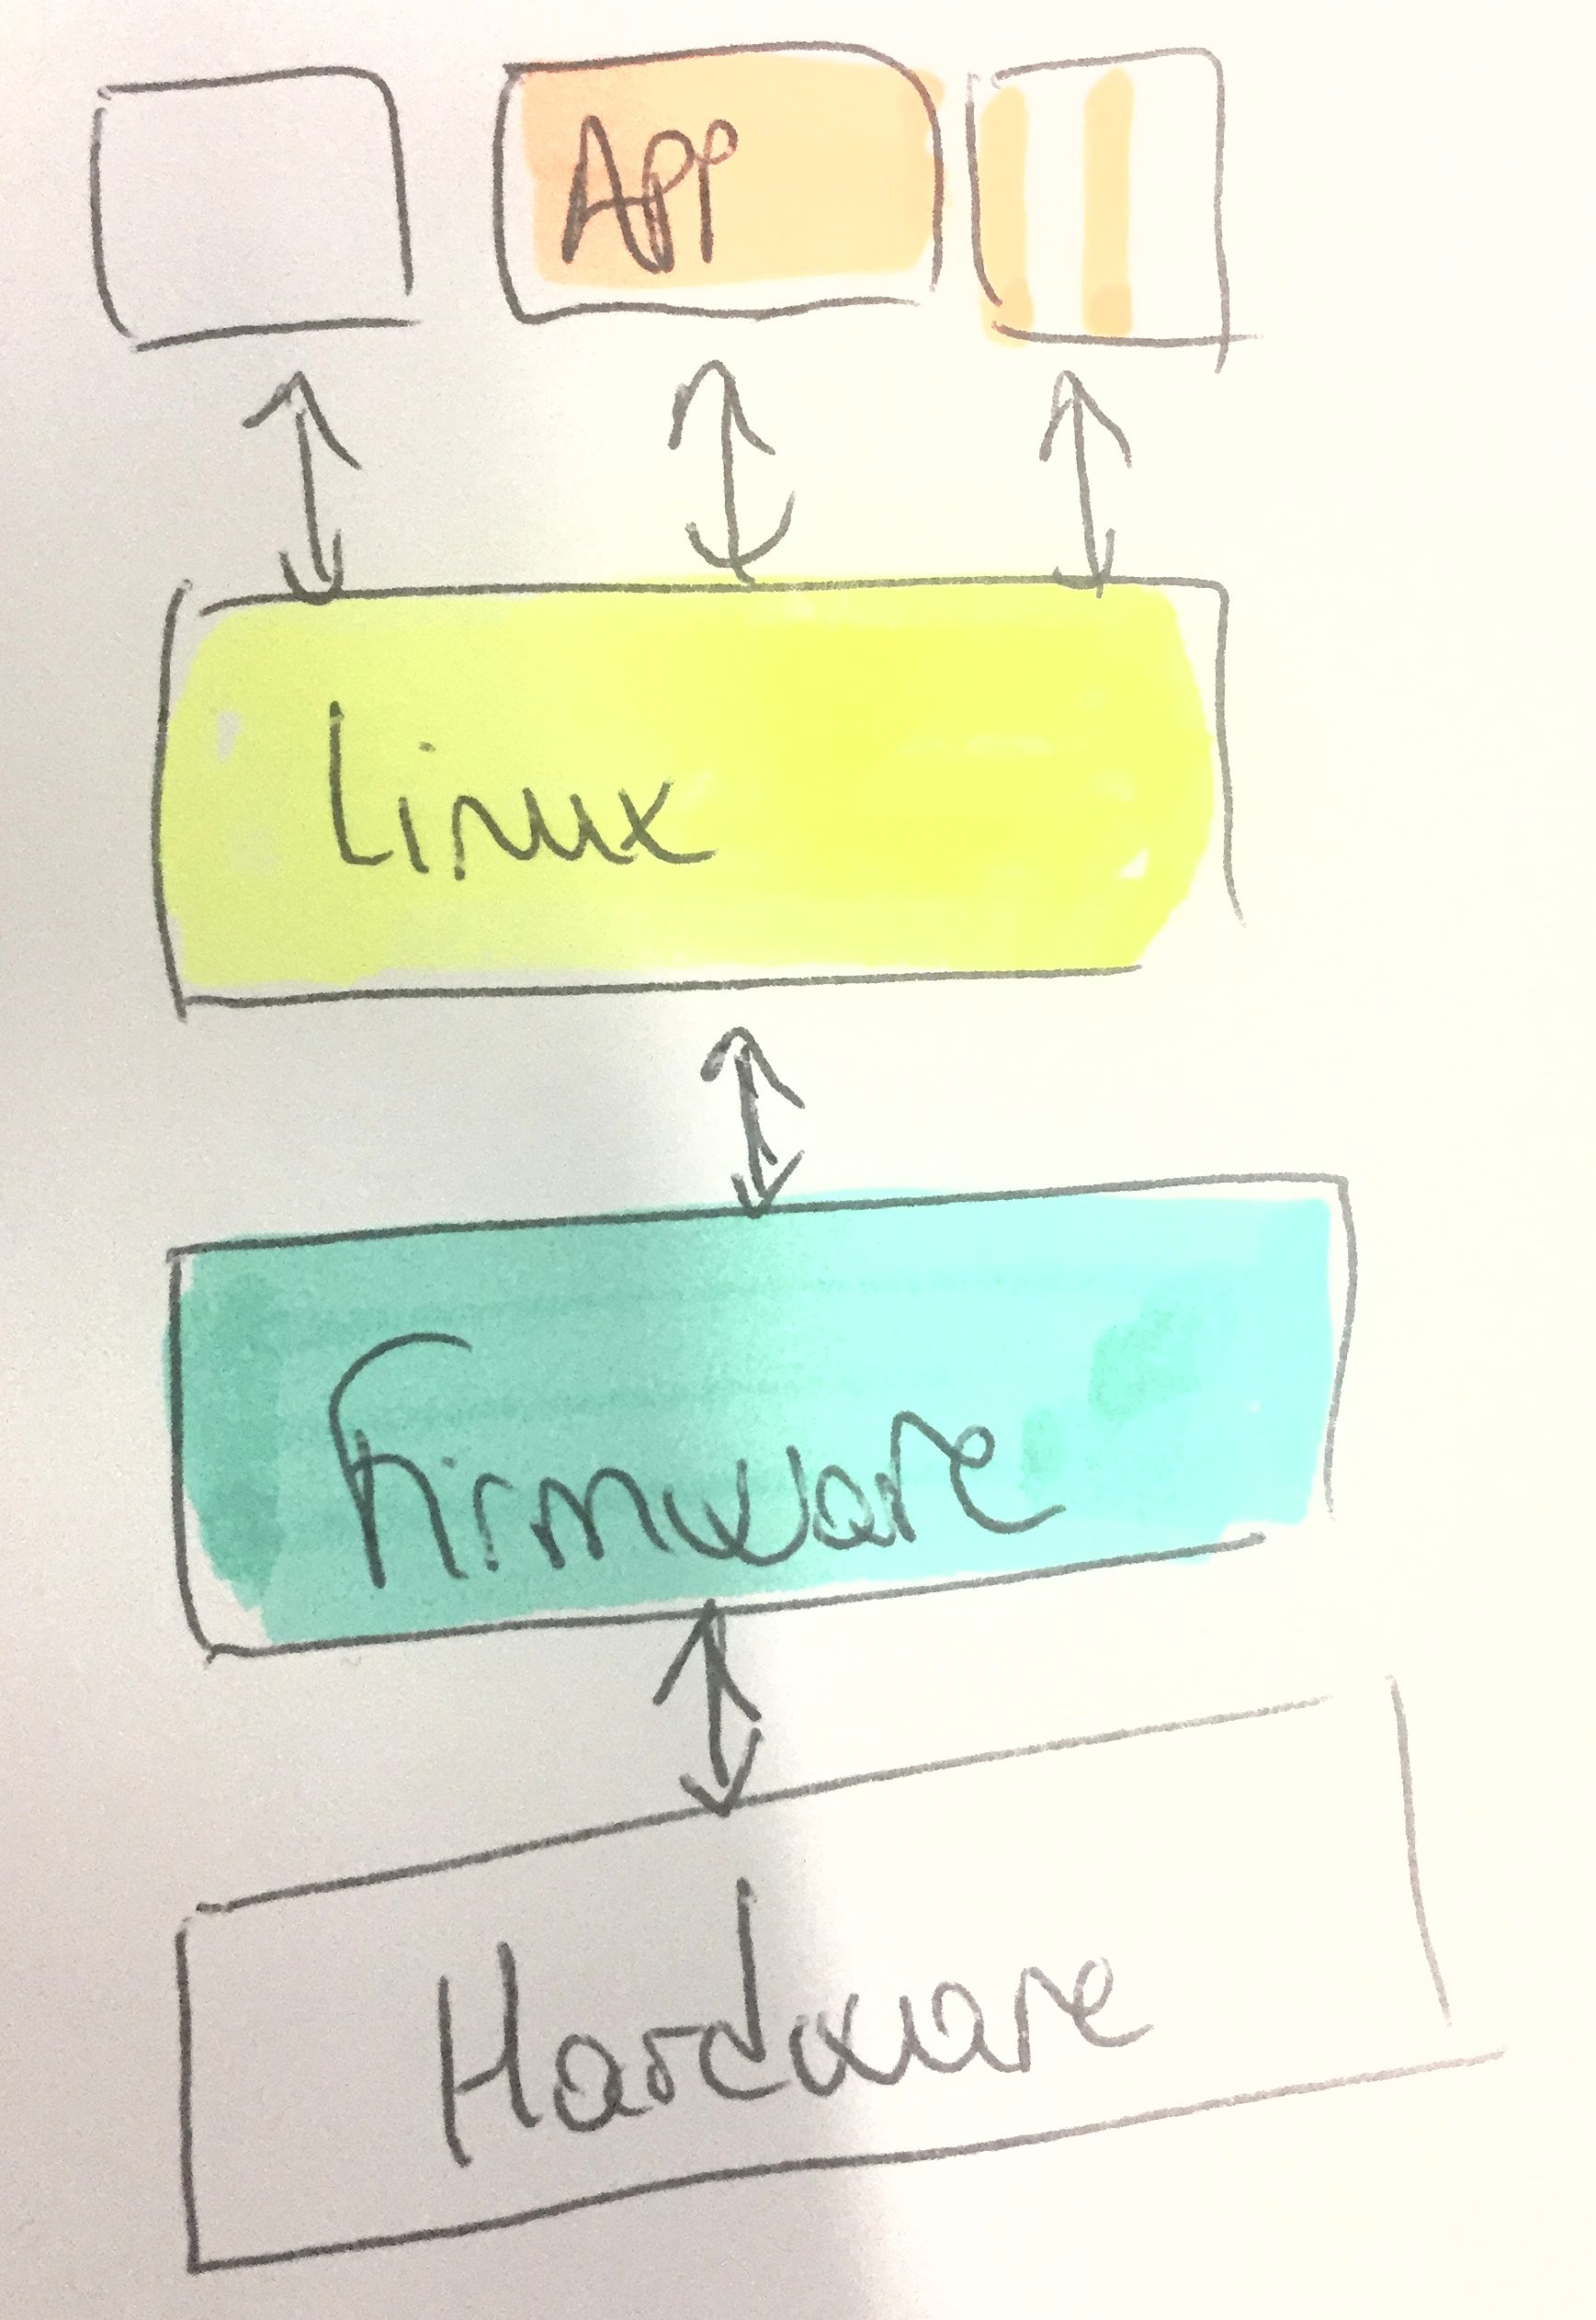
\includegraphics[width=0.3\textwidth]{Figures/computing-platform-1.jpg}
  \caption{Abstraction Layers of a Typical x86 Computing Platform}
  \label{fig:usecase:computing-platform}
\end{figure}

\begin{figure}
  \centering
  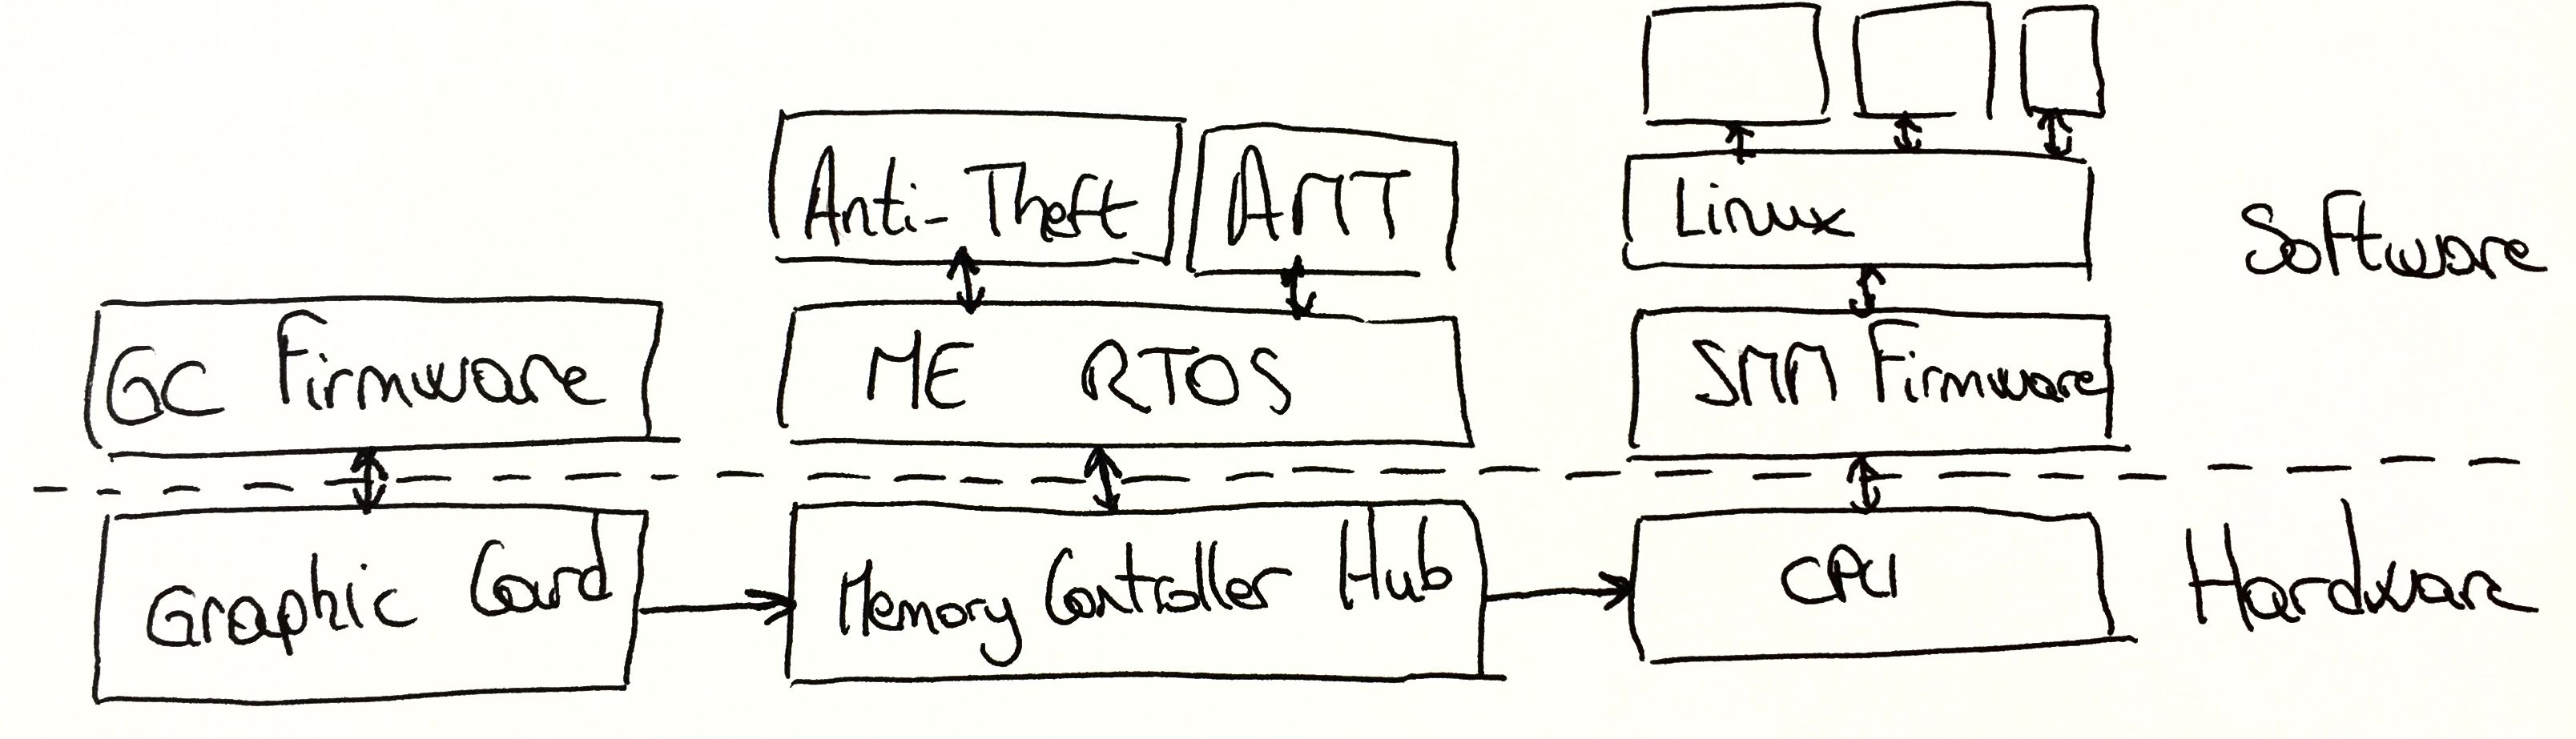
\includegraphics[width=0.8\textwidth]{Figures/intro-computing-platform.jpg}
  \caption{Multiple Software Stacks in x86 Hardware Architecture}
  \label{fig:usecase:computing-platform}
\end{figure}

\begin{figure}
  \centering
  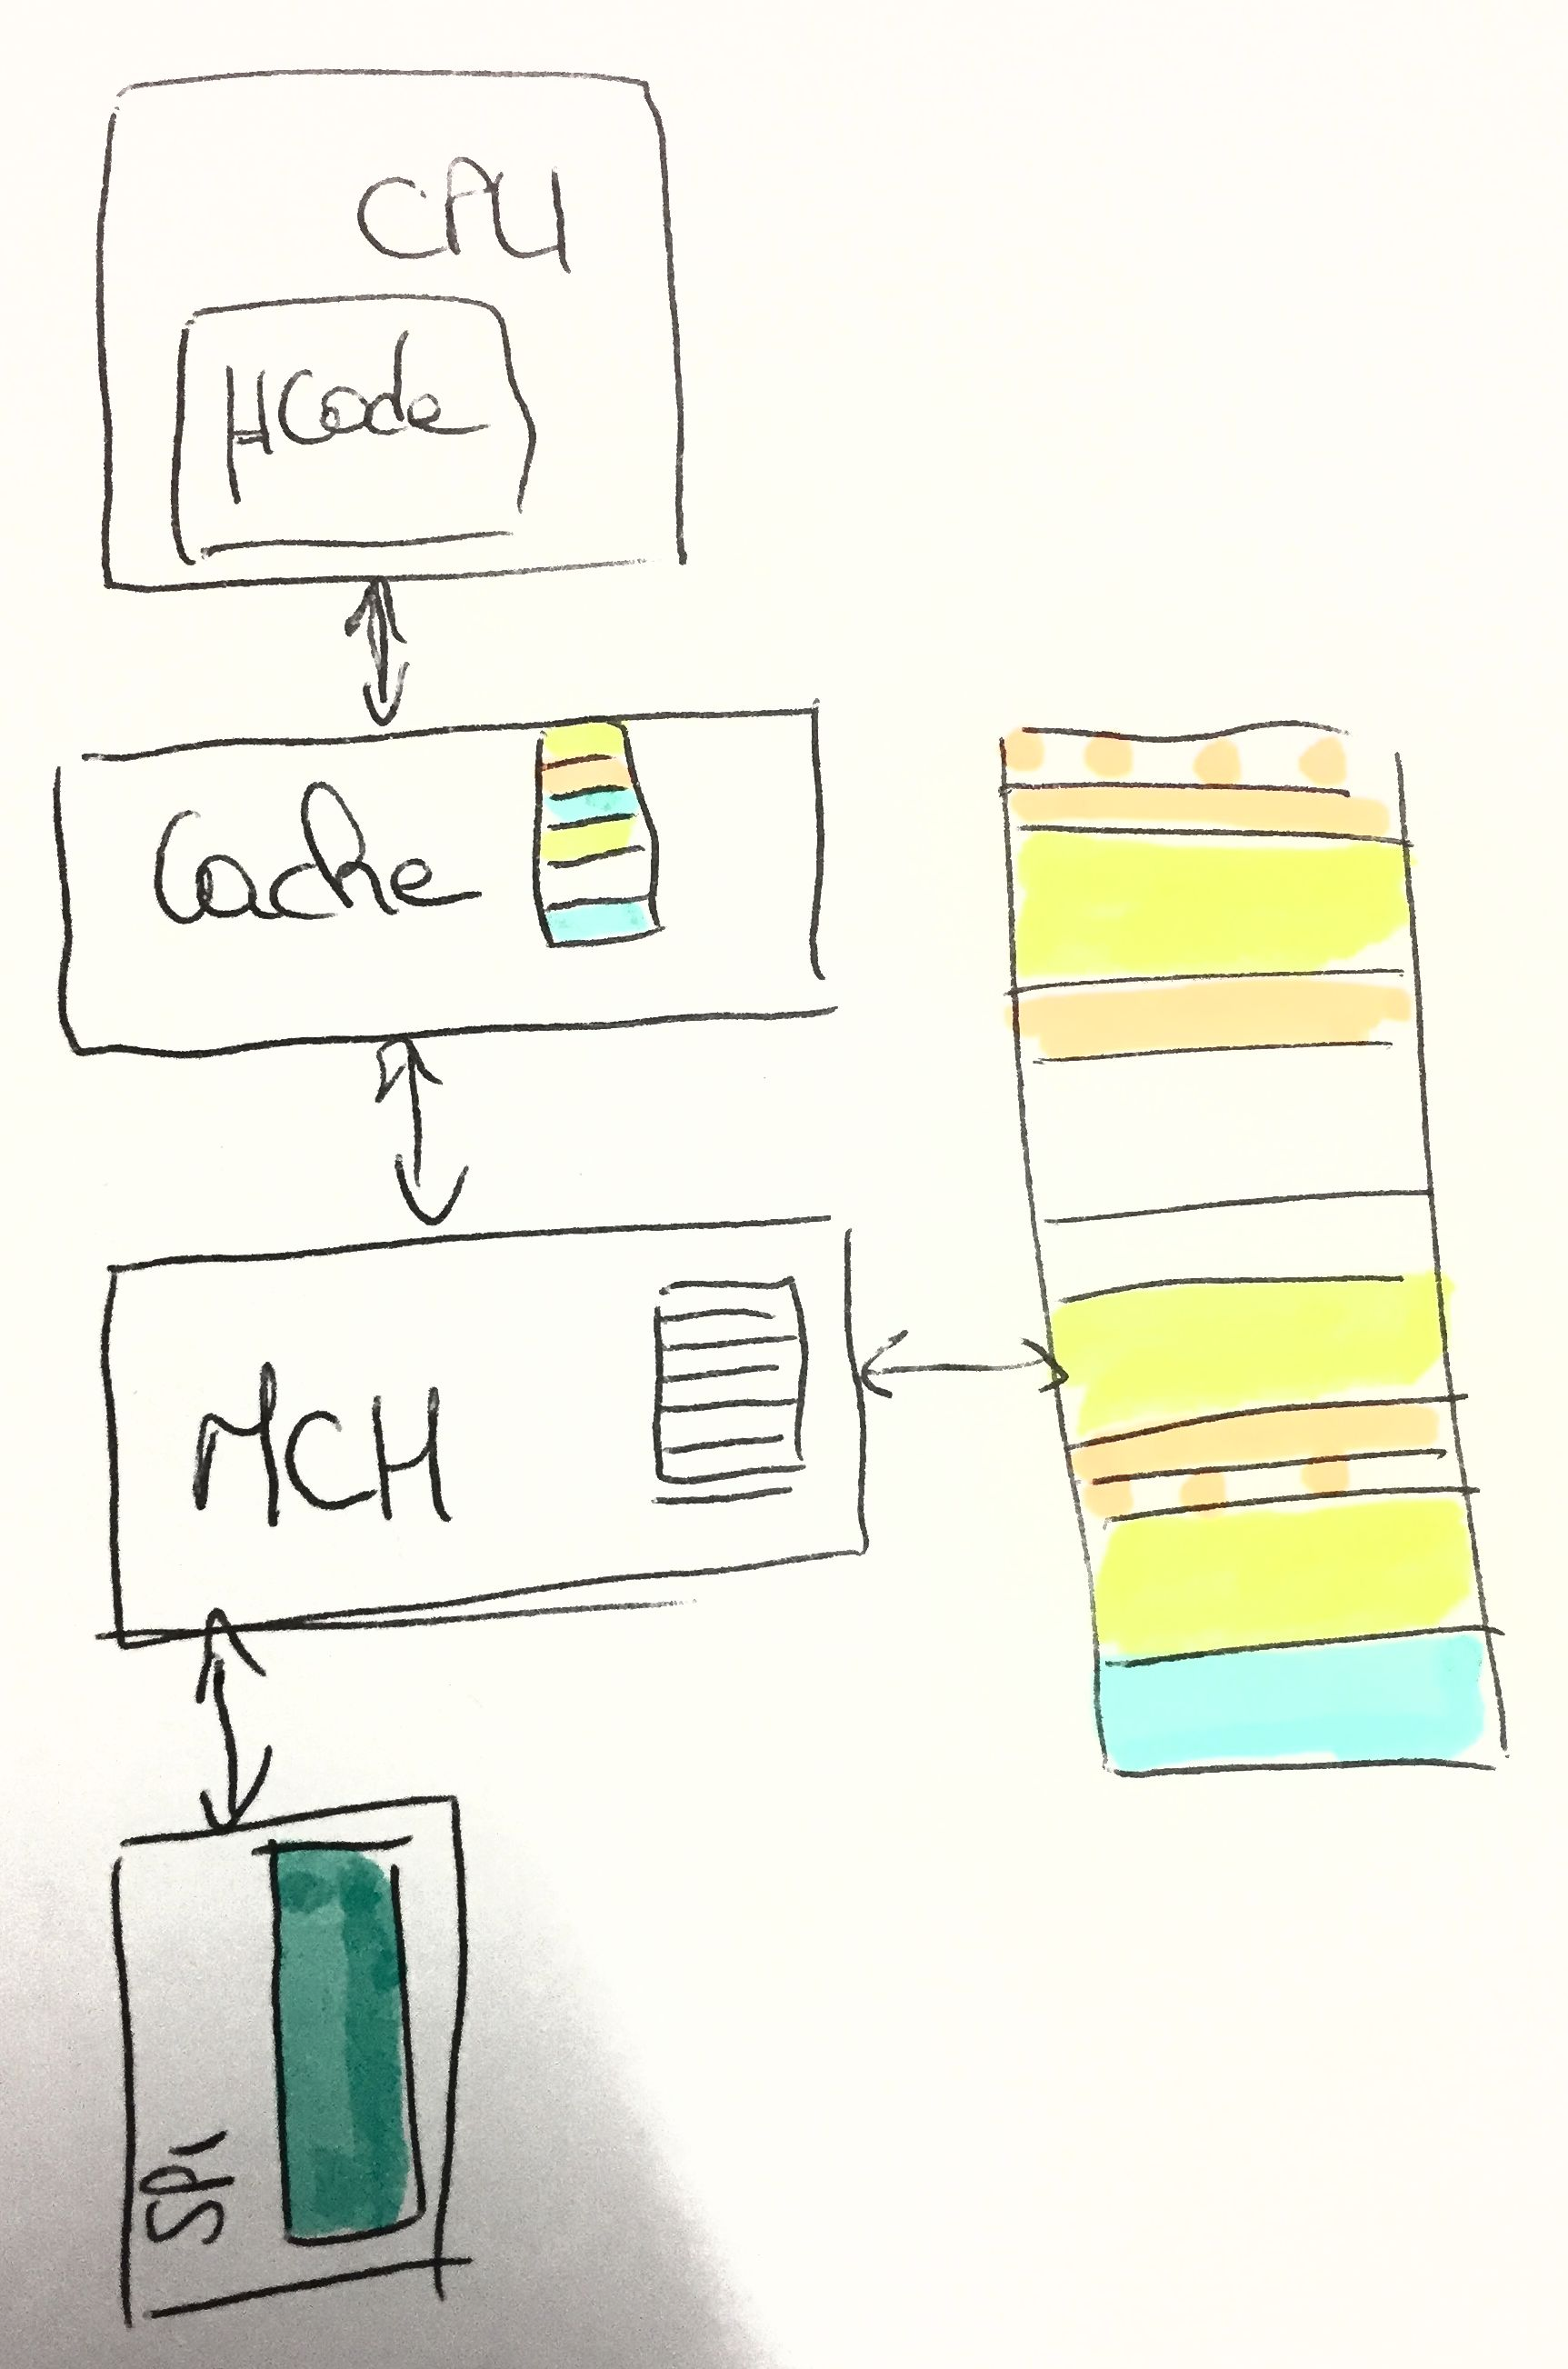
\includegraphics[width=0.3\textwidth]{Figures/computing-platform-3.jpg}
  \caption{Abstraction Layers of a Typical x86 Computing Platform}
  \label{fig:usecase:computing-platform}
\end{figure}

\section{Firmware}
\label{sec:usecase:firmware}

\section{Firmware HSE}
\label{sec:usecase:hse}

\section{Conclusion}
\label{sec:usecase:conclusion}
